\section{本章小结}
\label{sec:lp-summary}

回到章首的车间。等利润线在四边形上平移、最后停在角点，这幅图景在本章变成了三个可以计算的结论，它们的关系如图~\ref{fig:lp-summary-map}。

\begin{BookInlineFigure}
 \centering
 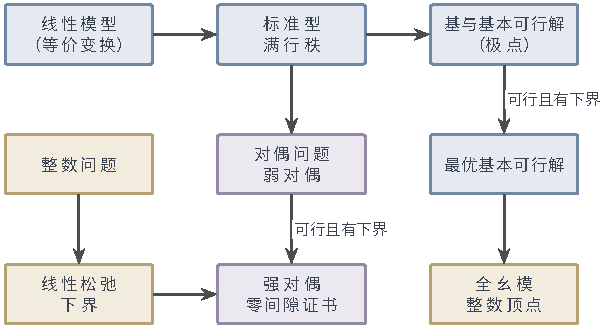
\includegraphics[width=102mm]{figures/05-optimization/01-linear-programming/tikz/lp-summary-map/figure.pdf}
 \caption{本章各部分的关系。蓝色框是原始问题的结构，紫色框是对偶与证书，黄色框是整数问题。箭头旁的文字是结论成立所需的条件。}
 \label{fig:lp-summary-map}
\end{BookInlineFigure}

第一，形式的统一。各种线性模型经过等价变换都能写成标准型，改写时松弛变量一一对应地保留可行集的形状，自由变量的分解保留最优值却可能多出角点。检查等式相容并删去冗余行之后，$\bm{A}$满行秩，基矩阵才有定义。

第二，解的位置。基本可行解就是可行集的极点，它由一个可逆的基矩阵解出；标准型只要可行且最优值有限，最优解就能在这有限个点中取得。非退化时换基对应沿边走到相邻顶点，退化时换基可能不移动，$\bm{u}\leq\bm{0}$时则得到无界可行方向。这个顶点结论依赖非负约束排除直线，含直线的多面体没有极点。

第三，解的证据。给约束配权重得到对偶问题，弱对偶说明对偶间隙等于$\bm{x}^\top\bm{s}$，因而非负，强对偶说明间隙可以精确为零。一对可行点满足互补松弛，就是最优性的完整证书，核对它只需矩阵乘法。表~\ref{tab:lp-summary}把这些结论和条件放在一起。

\begin{BookInlineTable}
 \centering
 \begin{tabular}{ll}
  \toprule
  结论 & 所需条件 \\
  \midrule
  基本可行解等于极点 & $\bm{A}$满行秩 \\
  存在最优基本可行解 & 标准型可行，最优值有限 \\
  沿边到不同的相邻顶点 & 基分量全为正，$\bm{u}$有正分量 \\
  弱对偶 & 两侧都可行 \\
  强对偶，对偶最优解存在 & 原始可行，最优值有限 \\
  松弛给出下界 & 最小化问题 \\
  顶点都是整数 & $\bm{A}$全幺模，$\bm{b}$是整数 \\
  \bottomrule
 \end{tabular}
 \caption{本章主要结论及其条件。}
 \label{tab:lp-summary}
\end{BookInlineTable}

整数问题是另一类问题。线性松弛提供一个界；全幺模配合整数右端保证顶点是整数，网络问题属于这一类；一般情形下松弛解可能是分数，恢复可行解需要针对具体结构论证可行性和误差。

本章说明了最优解在哪里、怎样核实，但没有给出高效的求解方法。第~\ref{chap:simplex-method}章沿着基本可行解换基前进，直到拿到零间隙证书。第~\ref{chap:lp-interior-point}章从可行集内部出发，保持$\bm{x}$和$\bm{s}$为正，逐步缩小互补松弛的残差。
